\textbf{6-1} 汽车在后轮的推动下，以加速度 $a$ 在地面上沿直线前进。已知汽车前轮与后轮的间距为 $2l$，质心位于前后轮的中央，离地高度为 $h$，后轮与地面之间的摩擦系数为 $\mu$，前轮为非驱动轮，与地面的摩擦可略。试问：$\mu$ 至少为多大时，后轮不致打滑？

\begin{center}
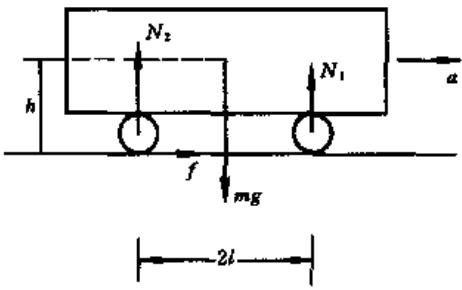
\includegraphics[width=0.2\textwidth]{figures/力图6-1-1.jpg}
\end{center}
\vfill

\textbf{6-2} 如力图6-2-1，质量为 $m$ 的均匀圆柱体，截面半径为 $R$，长为 $2R$。试求：圆柱体绕通过质心及两底面边缘的转轴的转动惯量。

\begin{center}
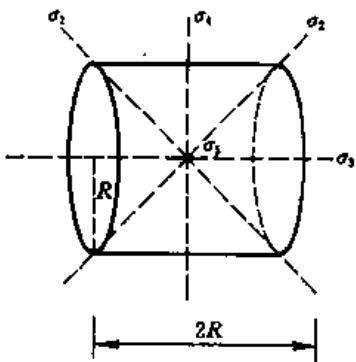
\includegraphics[width=0.2\textwidth]{figures/力图6-2-1.jpg}
\end{center}
\vfill

\newpage
\textbf{6-3} 如力图6-3-1，长为 $l$ 的均匀细杆水平地放置在桌面上，质心离桌边缘的距离为 $b$，从静止下落。已知杆与桌边缘之间的摩擦系数为 $\mu$。试求杆开始滑动时的角度 $\theta_C$。

\begin{center}
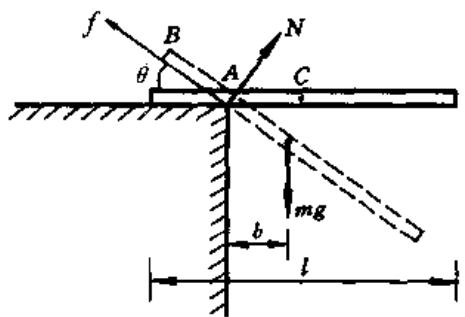
\includegraphics[width=0.2\textwidth]{figures/力图6-3-1.jpg}
\end{center}
\vfill

\textbf{6-4} 如力图6-4-1，实心圆柱体从桌边由静止下滚，圆柱体与桌边之间的摩擦系数为 $\mu$。圆柱体下滚过程中所转过的角度用 $\theta$ 表示。试求圆柱体开始相对桌边滑动时相应角度 $\theta$ 所满足的关系式，并用图解法在图上标出这个角度以及不滑动的转角范围。

\begin{center}
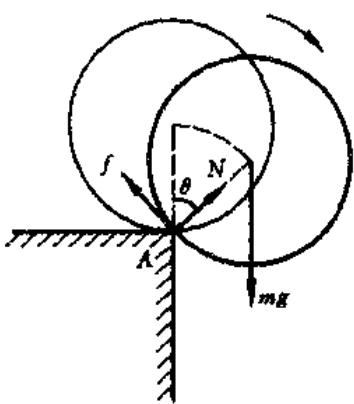
\includegraphics[width=0.2\textwidth]{figures/力图6-4-1.jpg}
\end{center}
\vfill

\newpage
\textbf{6-5} 如力图6-5-1，均匀细麦杆长 $l$，可绕通过中心 $O$ 的固定水平轴在铅垂面内自由转动。开始时麦杆静止于水平位置。一质量与麦杆相同的甲虫以速度 $v_{0}$ 垂直落到麦杆的 $\dfrac{1}{4}$ 长度处，落下后立即向端点爬行。

试问：1. 为使麦杆以均匀的角速度转动，甲虫沿麦杆爬行的速度应是多少？2. 甲虫轨迹的参变方程是什么？3. 为了使甲虫在麦杆转到铅直位置前能爬到端点，甲虫下落速度 $v_{0}$ 的最高值是多少？

\begin{center}
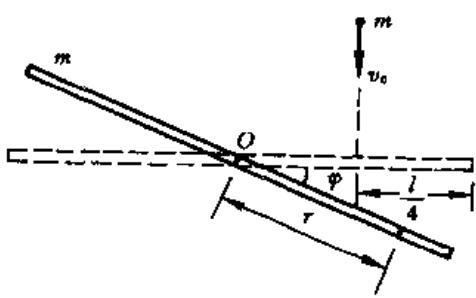
\includegraphics[width=0.2\textwidth]{figures/力图6-5-1.jpg}
\end{center}
\vfill

\textbf{6-6} 如力图6-6-1，半径为 $R$ 的均匀实心圆柱体在水平地面上作纯滚动，其中心 $O$ 点的速度为 $v_{0}$，它向前滚动时遇到一个高为 $h$ 的台阶，并发出完全非弹性碰撞。设圆柱和台阶前缘之间的摩擦系数足够大。

试问：1. $v_{0}$ 为何值时圆柱体能不脱离 A 点而滚上台阶继续前进？2. 对台阶高度 $h$ 有什么限制？

\begin{center}
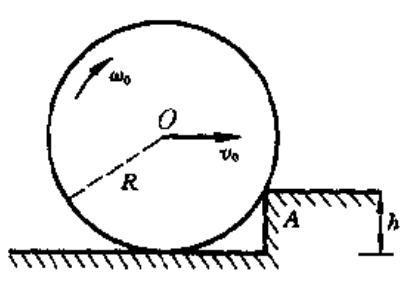
\includegraphics[width=0.2\textwidth]{figures/力图6-6-1.jpg}
\end{center}
\vfill

\newpage

\textbf{6-7} 如力图6-7-1，地球和月球的质量分别为 $M_{E}$ 和 $M_{m}$ ,两者中心的距离用 r 表示,月球可看作质点．设地球的自转轴和月球绕地球作圆周运动的转轴重合，都通过地球中心，地球和月球的角速度分别为 $\omega_{E}$ 和 $\omega_{m}$ ．由于潮汐运动，地球自转角速度会发生微小变化，从而地球和月球的间距以及地球和月球系统的总能量也将发生变化．

1. 试证明, 地球和月球间距的时间变化率 $\dot{r}$ 与地球自转角速度的时间变化率 $\omega_{E}$ 的关系为

$$
\dot {r} = - \frac {2 \sqrt {r} I _ {\mathrm{E}}}{M _ {\mathrm{m}} \sqrt {G M _ {\mathrm{E}}}} \dot {\omega} _ {\mathrm{E}}
$$

式中 $I_{E}$ 是地球对自转轴的转动惯量, G 是引力常量.

2. 试导出地球和月球系统机械能时间变化率的表达式。

3. 设现在的地球与月球间距为 $r(0)$ , 地球的自转角速度为 $\omega_{\mathrm{E}}(0)$ , 受扰动后相应的量变为 $r(t)$ 和 $\omega_{\mathrm{E}}(t)$ , 因扰动很小, 月球仍作圆周运动. 试证明

$$
\omega_ {\mathrm{E}} (t) = \omega_ {\mathrm{E}} (0) - \frac {M _ {\mathrm{m}} \sqrt {G M _ {\mathrm{E}}}}{I _ {\mathrm{E}}} [ \sqrt {r (t)} - \sqrt {r (0)} ]
$$

试计算地球和月球间距增加2\%时, 地球日将变成多少小时.

\begin{center}
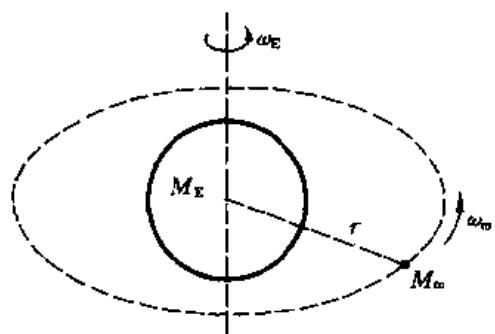
\includegraphics[width=0.25\textwidth]{figures/力图6-7-1.jpg}
\end{center}
\vfill
\newpage

\textbf{6-8} 某行星相对其质心轴的转动惯量为 $I$ ，自转角速度为 $\Omega$ 。质量为 $m$ 的卫星（可看作质点）绕该行星沿圆轨道运动，轨道半径为 $r$ ，角速度为 $\omega$ ，假定两种角速度的方向一致。

1. 一般情形下 $\Omega$ 与 $\omega$ 并不相等, 由于行星上的潮汐摩擦, 行星自转角速度将发生变化, 卫星的圆运动角速度也将相应地改变, 试求两种角速度的改变量之间的关系.

2. 潮汐摩擦将引起行星与卫星系统机械能的损耗, 试问在什么情形下系统机械能可达稳定值.
\vfill


\textbf{6-9} 如力图6-9-1，一线轴质量为 $m$ ，绕质心轴的转动惯量为 $I$ ，大小半径分别为 $R$ 和 $r$ ，轴上绕线，以力 $F$ 拉线，拉力方向与水平面的夹角用 $\theta$ 表示。线轴放置在水平桌面上，与桌面之间的摩擦系数为 $\mu$ ，试讨论线轴的运动情况。

\begin{center}
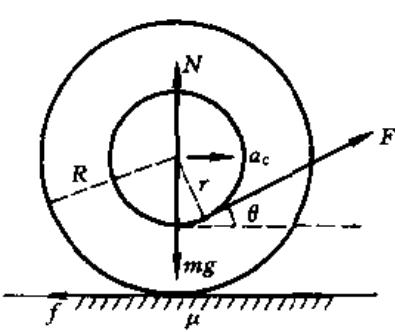
\includegraphics[width=0.2\textwidth]{figures/力图6-9-1.jpg}
\end{center}
\vfill
\newpage

\textbf{6-10} 如力图6-10-1，在 $\alpha = 30^{\circ}$ 的斜面上，质量 $m_{2} = 4\mathrm{kg}$ 的木块经轻绳与质量 $m_{1} = 8\mathrm{kg}$ 半径 $r = 5\mathrm{cm}$ 的实圆柱体的转轴相连。已知斜面的摩擦系数 $\mu = 0.2$ ，圆柱体轴承中的摩擦可以忽略。试求物体的加速度 $a$ ，并讨论加速度 $a$ 、张力 $T$ 、圆柱体所受摩擦力 $f_{1}$ 随斜面倾角 $\alpha$ 的变化。

\begin{center}
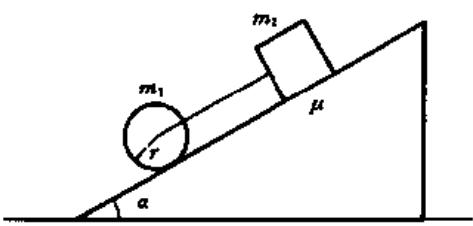
\includegraphics[width=0.25\textwidth]{figures/力图6-10-1.jpg}
\end{center}
\vfill


\textbf{6-11} 如力图6-11-1，半径为 $R$ 的乒乓球，绕质心轴的转动惯量 $I = \frac{2}{3} mR^2, m$ 为乒乓球的质量，以一定的初始条件在粗糙的水平面上运动。开始时球的质心速度为 $v_{\mathrm{C0}}$ ，初角速度为 $\omega_0$ ，两者的方向如图所示。已知乒乓球与地面之间的摩擦系数为 $\mu$ 。试求乒乓球开始作纯滚运动所需的时间及纯滚时的质心速度。

\begin{center}
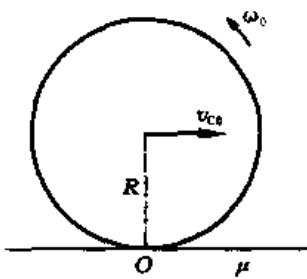
\includegraphics[width=0.2\textwidth]{figures/力图6-11-1.jpg}
\end{center}
\vfill
\newpage

\textbf{6-12} 如力图6-12-1，实心圆柱体从高度为 $h$ 的斜坡上从静止纯滚动地到达水平地面上, 继续纯滚动, 与光滑竖直墙作完全弹性碰撞后返回, 经足够长的水平距离后重新作纯滚动, 并纯滚动地爬上斜坡. 设地面与圆柱体之间的摩擦系数为 $\mu$ , 试求圆柱体爬坡所能达到的高度 $h'$ .

\begin{center}
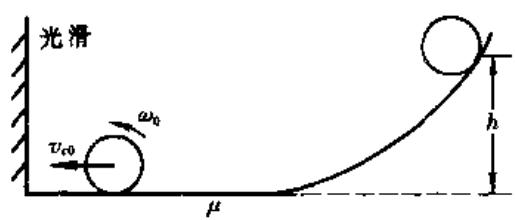
\includegraphics[width=0.3\textwidth]{figures/力图6-12-1.jpg}
\end{center}
\vfill

\textbf{6-13} 如力图6-13-1，实心均匀小球自圆柱面的顶端从静止下滚.

1. 为了保证在 $\varphi \leqslant 45^{\circ}$ 的范围内小球作纯滚动, 试问摩擦系数 $\mu$ 至少应为多少.

2. 设 $\mu = 0.7$ , 试求纯滚结束时小球的质心速度 $v_{1}$.

3. 试求小球从圆柱面脱离时小球的位置 (用 $\varphi$ 角表示) 所满足的方程 (不必求解).

\begin{center}
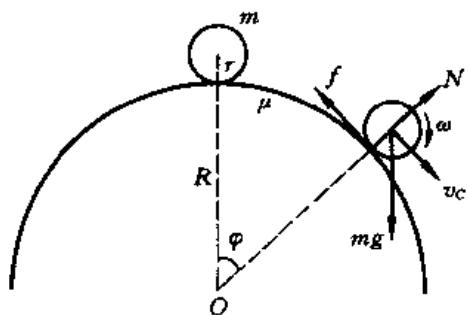
\includegraphics[width=0.25\textwidth]{figures/力图6-13-1.jpg}
\end{center}
\vfill
\newpage

\textbf{6-14} 在水平地面上有两个完全相同的均匀实心球，其一作纯滚动，质心速度为 $v$ ，另一静止不动。两球作完全弹性碰撞，因碰撞时间很短，碰撞过程中摩擦力的影响可以忽略不计。

试求: 1. 碰后两球达到纯滚时的质心速度. 2. 全部过程中损失的机械能的百分数.
\vfill


\textbf{6-15} 如力图6-15-1，两个质量和半径均相同的实心圆柱轮，它们的质心轴互相平行，并用一轻杆相连，轴与轴承间的摩擦忽略不计。两轮先以共同的初速 $v_{0}$ 沿水平方向运动，两轮的初角速度为零。然后同时轻轻与地面相接触。设两轮与地面之间的摩擦系数分别为 $\mu_{1}$ 和 $\mu_{2}(\mu_{1}>\mu_{2})$ 。试求两轮均变为纯滚动所需的时间及纯滚后的平动速度。

\begin{center}
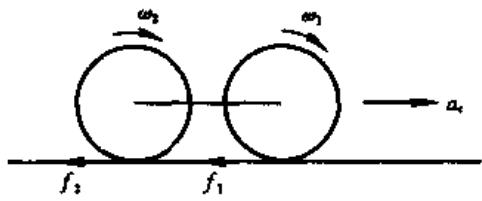
\includegraphics[width=0.3\textwidth]{figures/力图6-15-1.jpg}
\end{center}
\vfill
\newpage

\textbf{6-16} 如力图6-16-1，一半径为 $R$ 的实心均匀球，开始时质心静止，但绕通过质心的水平轴以角速度 $\omega_{0}$ 旋转，在重力作用下垂直下落到地面，球上最低点离地面的高度为 $h$。球与地面碰撞的恢复系数为 $e$，球与地面之间的摩擦系数为 $\mu$ ，忽略空气阻力及碰撞时产生的形变。

1. 试求碰地后球的质心速度和自转角速度。

2. 试求第一次落地点与第二次落地点之间的水平距离。

3. 试画出碰后球的质心速度与地面夹角 $\theta$ 的正切与初始角速度 $\omega_0$ 的关系曲线。

\begin{center}
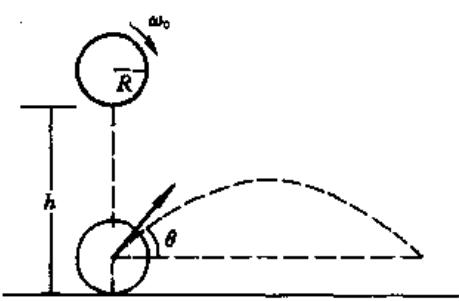
\includegraphics[width=0.25\textwidth]{figures/力图6-16-1.jpg}
\end{center}
\vfill


\textbf{6-17} 如力图6-17-1，斜面体放置在光滑水平面上，斜面倾角为 $\theta$ ，一半径为 $R$ 的圆柱体在斜面上无滑动地下滚。设斜面体和圆柱体具有相同的质量 $m$ ，试求斜面体的加速度。

\begin{center}
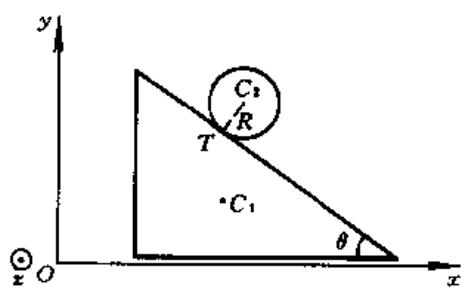
\includegraphics[width=0.25\textwidth]{figures/力图6-17-1.jpg}
\end{center}
\vfill
\newpage

\textbf{6-18} 如力图6-18-1，实心球在水平面内运动，质心的初始速度为 $\nu_{0}$ , 绕质心 $C$ 转动的初始角速度为 $\omega_{0}$ , 球与水平面之间的摩擦系数为 $\mu$ . 试分析球在水平面内的运动.

\begin{center}
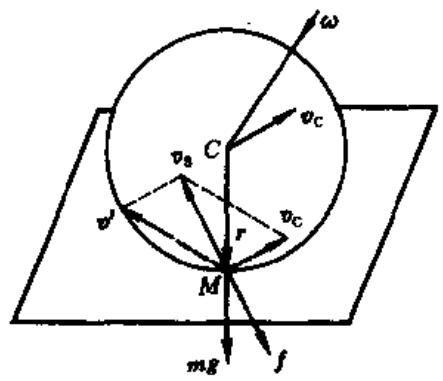
\includegraphics[width=0.2\textwidth]{figures/力图6-18-1.jpg}
\end{center}
\vfill


\textbf{6-19} 如力图6-19-1，一个质量为 $m$ , 半径为 $R_A$ 的均匀圆盘 $A$ 在光滑水平面 $Oxy$ 内以速度 $V$ 沿 $x$ 方向平动, 圆盘中心至 $x$ 轴的垂直距离为 $b$ . 圆盘 $A$ 与另一静止的、其中心位于坐标原点 $O$ 的均匀圆盘 $B$ 相碰. 圆盘 $B$ 的质量与 $A$ 相同, 半径为 $R_B$ . 假定碰撞后两圆盘接触处的切向速度分量相等, 并假定碰撞前、后两盘沿连心线方向的相对速度大小不变. 试求:

1. 碰后两圆盘质心速度的 $x$ 分量和 $y$ 分量 $V_{Ax}^{\prime}, V_{Ay}^{\prime}, V_{Bx}^{\prime}, V_{By}^{\prime}$ .

2. 碰后两圆盘的动能 $E_A'$ 和 $E_B'$ .

\begin{center}
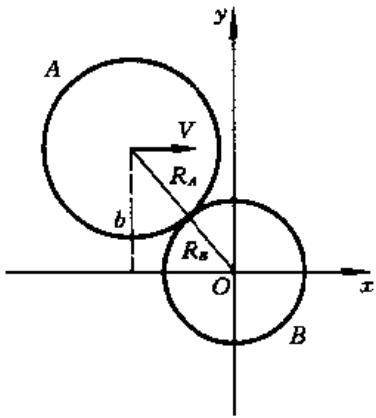
\includegraphics[width=0.2\textwidth]{figures/力图6-19-1.jpg}
\end{center}
\vfill
\newpage

\textbf{6-20} 如力图6-20-1，均匀细圆环半径为 $R$ ，质量为 $m$ ，平放在水平桌面上，与桌面之间的摩擦系数为 $\mu$ 。圆环质心 $O$ 沿 $x$ 轴以初速 $v_{\mathrm{C}0}$ 运动，同时圆环绕质心以初角速度 $\omega_0$ 顺时针转动， $v_{\mathrm{C}0}$ 与 $\omega_0$ 满足 $v_{\mathrm{C}0} = R\omega_0$ 。

试求: 1. 圆环所受摩擦力及摩擦力对质心的力矩. 2. 从开始到圆环停止运动所需时间.

\begin{center}
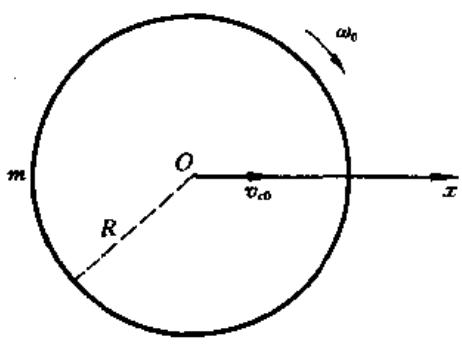
\includegraphics[width=0.25\textwidth]{figures/力图6-20-1.jpg}
\end{center}
\vfill


\textbf{6-21} 长为 $l$ 的均匀细杆竖直地放置在光滑地面上，从静止倒下．试求落到地面时的质心速度.
\vfill
\newpage


\textbf{6-22} 如力图6-22-1，光滑水平地面上静止地放着质量为 $M$ 、长为 $l$ 的均匀细杆。质量为 $m$ 的质点以垂直于杆的水平初速 $\upsilon_0$ 与杆的一端作完全弹性碰撞.

试求: 1. 碰后系统质心的速度及绕质心的角速度. 2. 实际的转轴(即静止点)位于何处.

\begin{center}
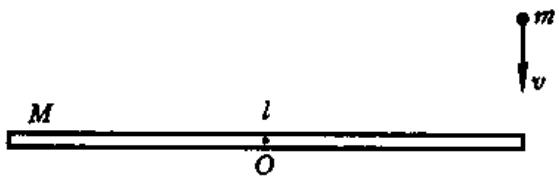
\includegraphics[width=0.3\textwidth]{figures/力图6-22-1.jpg}
\end{center}
\vfill


\textbf{6-23} 如力图6-23-1，长为 $2l$ 的均匀细杆，下端支在地面上，上端靠在竖直墙上，从静止下滑，开始时杆与地面的夹角为 $\theta_0$ 。设杆与地和墙之间的摩擦可略。试问质心下降到初始高度的几分之几时，杆的上端与墙脱离。

\begin{center}
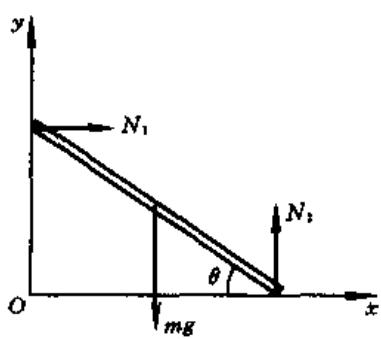
\includegraphics[width=0.25\textwidth]{figures/力图6-23-1.jpg}
\end{center}
\vfill
\newpage

\textbf{6-24} 如力图6-24-1，在光滑地面上静止地放置着两根质量均为 $m$ ，长度均为 $l$ 的均匀细杆.其中一杆由相等的两段构成，中间用光滑的铰链连接起来.在两杆的一端，各施以相同的垂直于杆的水平冲量 $J$ .试求两杆所获动能之比.

\begin{center}
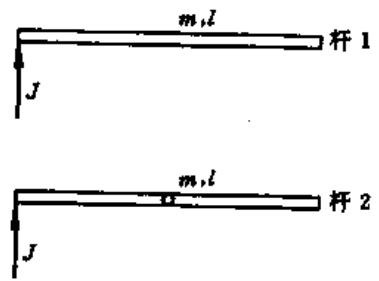
\includegraphics[width=0.25\textwidth]{figures/力图6-24-1.jpg}
\end{center}
\vfill


\textbf{6-25} 如力图6-25-1，半径为 $R$ 的圆环绕铅垂的直径轴以角速度 $\omega$ 匀角速旋转。一细杆长 $L = \sqrt{2} R$ , 其两端约束在圆环上可作无摩擦滑动, 细杆的位置用 $OC$ 与铅垂轴的夹角 $\theta$ 表示, $C$ 为细杆的质心。试求细杆在圆环上的平衡位置, 并讨论平衡的稳定性。

\begin{center}
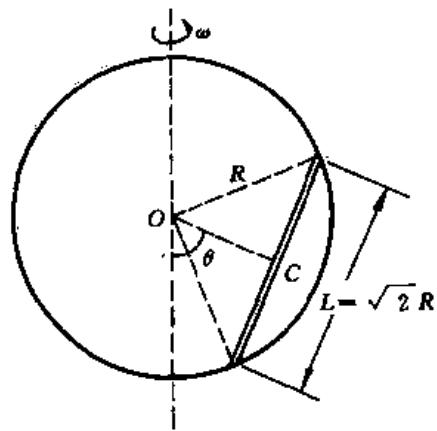
\includegraphics[width=0.2\textwidth]{figures/力图6-25-1.jpg}
\end{center}
\vfill
\newpage

\textbf{6-26} 如力图6-26-1， $Ox$ 和 $Oy$ 分别是支架的水平臂和铅垂臂， $Ox$ 臂绕铅垂臂作匀角速转动，角速度为 $\omega$ 。一均匀细杆的两端 $A$ 和 $B$ 被分别约束在两臂上运动，假定约束是理想的，细杆的质量为 $m$ ，长为 $2L$ ，细杆位置用图中 $\theta$ 角表示， $\theta$ 角是 $OC$ 与 $Oy$ 之间的夹角， $C$ 为细杆质心。以支架为参考系考察细杆的运动。

1. 试写出细杆的能量表达式。2. 试求细杆的平衡位置，并讨论平衡的稳定性。

\begin{center}
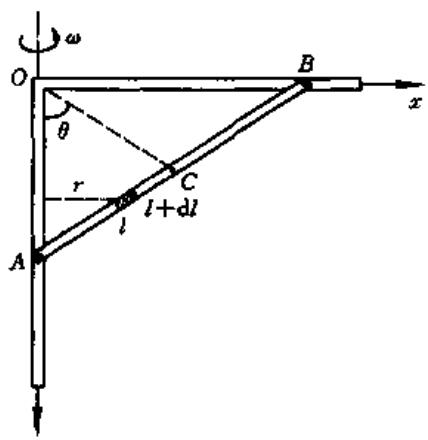
\includegraphics[width=0.2\textwidth]{figures/力图6-26-1.jpg}
\end{center}
\vfill


\textbf{6-27} 1. 如力图6-27-1，质量为 $m$ 的陀螺绕对称轴高速旋转, 角速度为 $\omega$ , 绕对称轴的转动惯量为 $I$ , 质心到转轴下端的距离为 $l_{\mathrm{C}}$ , 在重力矩的作用下, 陀螺将绕竖直轴作缓慢进动. 试求进动角速度的近似值.

2. 若转轴下端与桌面是面接触, 并受摩擦力的作用. 试解释在摩擦的作用下, 转轴将产生趋向于竖直轴的附加运动, 并计算从倾斜 $\theta$ 角到竖直位置所需的时间.

\begin{center}
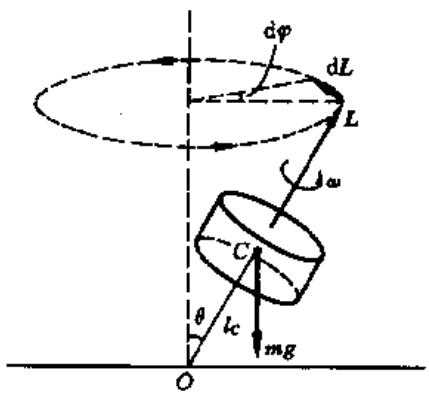
\includegraphics[width=0.25\textwidth]{figures/力图6-27-1.jpg}
\end{center}
\vfill

